\documentclass[10pt]{article}
\usepackage[a4paper, margin=1in]{geometry}
\usepackage{newtxtext, newtxmath}
\usepackage{graphicx, booktabs, array, xcolor, caption, enumitem, amsmath}
\usepackage[section]{placeins}
\usepackage[hidelinks]{hyperref}
\usepackage{xurl}
\sloppy
\captionsetup{font=small, labelfont=bf}
\setlist{nosep, leftmargin=1.4em}
\graphicspath{{figures/}}
\makeatletter\newcommand{\tabinput}[1]{\IfFileExists{#1}{\@@input #1 }{\textit{(pending)} \\}}\makeatother
\newcommand{\layerbest}[1]{\IfFileExists{tables/layer_best_#1.tex}{\input{tables/layer_best_#1.tex}}{(pending)}}

\title{\vspace{-6mm}\rule{\linewidth}{2pt}\\[3mm]
\textbf{Reproducing ``The Power of Prior'':\\Training-Free Open-Vocabulary Segmentation with LLaVA}\\[1mm]
\large A controlled reproduction and analysis on PASCAL VOC 2012\\[-1mm]\rule{\linewidth}{0.6pt}}
\author{\textbf{[Author names]}}
\date{}

\begin{document}
\maketitle
\vspace{-8mm}

\begin{abstract}
\noindent FSeg-LLaVA (Zhang et al., CVPR 2026) segments images without any segmentation training. It asks a frozen
LLaVA model whether each class is present, turns the similarity between the class-name token and the image tokens in
middle LLM layers into an activation map, and converts that map into point and box prompts for a frozen SAM. We
reimplemented the method in Hugging Face \texttt{transformers}, following the authors' released code where it differs
from the paper text, and evaluated it on all 1{,}449 PASCAL VOC 2012 validation images. All choices were made on a
separate 200-image tuning subset of the VOC \emph{train} split; validation was used only for reporting. \textbf{The
reproduction reaches 65.85 mIoU (VOC21), against 68.0 reported in the paper.} The component ablations move in the same
direction as the paper's tables. LLaVA's maps alone reach only 18.7 mIoU, so most of the final accuracy comes from SAM
prompted by them; replacing LLaVA's yes/no answers with the true class list would add 6.3 points. Reading the class
token's hidden state one position too early costs 17.3 points, which shows how localized the signal is. A layer-by-layer study reproduces the paper's layer ablation and refines it: maps from the
middle layers (7--13) are the most \emph{precise} (79\% of marked pixels correct) and therefore the best seeds for SAM,
while maps from layers 17--22 cover more of each object and score higher on their own but give SAM worse prompts. We also tested
six improvements (filters on LLaVA's answers, background rules, per-instance prompts, class-name aliases and a
combination). None transferred: the only tuning-set gain (+1.2) scored $-0.15$ on validation (95\% CI $-0.83$ to $+0.55$).
\end{abstract}

\section{Aim and contribution}
\textbf{Aim.} We aim to reproduce the proposed training-free segmentation framework and to investigate how spatial
information already encoded in a vision-language model can be used for open-vocabulary semantic segmentation without
task-specific fine-tuning.

\textbf{What this report adds} to the original paper, stated modestly:
\begin{enumerate}
\item An independent reimplementation in a different framework (\texttt{transformers} instead of the original LLaVA
code base), with every difference between the paper text and the released code made a switch and measured
(Table~\ref{tab:ablations}).
\item A controlled protocol: hyperparameters and design choices were selected on a held-out subset of VOC
\emph{train}; the validation set was run once per final configuration, with a paired bootstrap for differences.
\item An error decomposition: recognition (oracle class list), localization (LLaVA maps without SAM) and SAM
prompting, plus per-class results and recognition precision/recall.
\item A layer-by-layer measurement of where LLaVA's spatial information sits, separating map coverage from the precision
that SAM prompting needs (Section~\ref{sec:layers}).
\item Negative results for six improvement attempts, reported in full (Table~\ref{tab:tuning}).
\end{enumerate}

\section{Method}
For an image $I$ and each candidate class $c$, the method has three stages.

\textbf{Question--answer pipeline (QAP).} LLaVA-1.5 is asked a fixed two-sentence question (``Does the image have the
class of a $c$? Answer yes or no \ldots{} the first sentence is `yes, it contains a $c$.' the second sentence is to
describe the $c$.''). Classes answered ``no'' are dropped.

\textbf{Text--visual response (TVR).} For each class-name token $t_c$ in the answer, the cosine similarity between its
hidden state and every image-token hidden state is averaged over LLM layers $l_s..l_e$ (7..13 for Vicuna-7B), giving a
$24{\times}24$ map $\tilde D$. Locations below $\tau=\min(\alpha\max\tilde D, \beta)$ are zeroed ($\alpha=0.75$,
$\beta=0.19$). A second map comes from the description sentence: text-to-image attention maps of all (layer, head) pairs
are ranked by the entropy of their connected regions, the 30 lowest-entropy maps are averaged and thresholded at their
mean ($M_A$). A constant background score $\min(\alpha\max_c D_c, \beta)$ competes with the class maps in an argmax.

\textbf{Visual generation module (VGM) and SAM.} CLIP patch features give a foreground prototype per class and a
background prototype; locations closer to the class prototype form a refined mask $M_r$. Connected-component centroids
of $M_r$ (positive points), its bounding box, and the other classes' points become SAM prompts; SAM (ViT-H) runs three
refinement rounds, each fed the previous round's logits. Overlapping class masks fall back to LLaVA's argmax.

\textbf{Paper text versus released code.} Where the two differ, our default follows the released code
(\url{https://github.com/zbf1991/FSeg-LLaVA}): $M_A$ is combined with the thresholded map by a \emph{union} (the paper
writes a product, Eq.~8), the attention heads are filtered by attention mass ($>0.24$) before ranking, other classes'
points are passed to SAM with label $-1$, SAM is refined three times, and images are stretched (not padded) to a square.
Table~\ref{tab:ablations} measures the most consequential of these.

\section{Data}
\textbf{PASCAL VOC 2012 segmentation} (Everingham et al., IJCV 2010), downloaded from the official mirror
(\texttt{VOCtrainval\_11-May-2012.tar}, SHA-256 checked). Annotators labelled every pixel of the selected images with
one of 20 object classes or background; object boundaries and ambiguous regions are marked \emph{void} (255) and
ignored in scoring. The segmentation subset has 1{,}464 \emph{train} and 1{,}449 \emph{val} images; test labels are not
public. We use VOC21 scoring (20 classes plus background), with intersection and union accumulated over the whole set
before averaging over classes (the \texttt{mmseg} convention used by the paper).

\textbf{Preparation.} No training data is used. The 20 class names are queried for every image (no annotation is used
at inference). For tuning we drew 200 images from \emph{train} at random (seed 0; list in
\texttt{splits/voc\_train\_dev200.txt}); it is disjoint from validation. The oracle ablation is the only configuration
that reads labels at inference, and it is reported as an analysis, not as a result.

\section{Setup}
LLaVA-1.5-7B (Vicuna-7B with CLIP ViT-L/14-336, 576 image tokens) from the Hugging Face conversion
\texttt{llava-hf/llava-1.5-7b-hf}, fp16, greedy decoding (128 new tokens), slow SentencePiece tokenizer;
SAM ViT-H (\texttt{sam\_vit\_h\_4b8939}). One NVIDIA A30 (24\,GB). LLaVA runs once per image and all its outputs are
cached, so SAM-stage variants are cheap: tracing the validation set took 2\,h\,49\,min (7.0\,s per image for 20
classes); one SAM configuration takes about 9\,min.

\section{Results}
\subsection{Reproduction and ablations}
\begin{table}[h]
\centering\small
\caption{VOC21 mIoU. \emph{Tuning}: 200 VOC-train images. \emph{Val}: all 1{,}449 validation images, with the change
relative to the reproduction. \emph{Paper}: the corresponding entry of the paper's Tables 1, 4, 5 and 6 (LLaVA-1.5,
VOC val).}
\label{tab:ablations}
\begin{tabular}{lccc}
\toprule
Configuration & Tuning & Val & Paper \\
\midrule
\tabinput{tables/ablations.tex}
\bottomrule
\end{tabular}
\end{table}

\noindent The reproduction scores \textbf{65.85} on validation, 2.2 points below the paper. The ablations agree with the
paper in direction and order: box and points together beat either alone, and removing the attention mask or the
prototype step changes little. We could not locate the remaining gap. Plausible sources, none verified, are the
converted checkpoint and newer library versions (fp16 numerics differ), the authors' unreleased VOC class-name file,
and small differences in our port. Running the original code in its pinned environment would settle it.

Two rows are not in the paper. \textbf{The class-token state must be read at the class token itself}: reading the
state one position earlier (the token before the class name, e.g.\ ``a'') drops validation mIoU from 65.85 to 48.57.
\textbf{The paper's product formula is worse than the code's union} by 4.2 points.

\subsection{Where the accuracy comes from}
LLaVA's maps on their own, without SAM, reach 18.7 mIoU: they mark the right object but cover only part of it
(Figure~\ref{fig:success}, third column). SAM, prompted by points and a box derived from those maps, adds 47 points.
Recognition is the largest remaining loss. With the true class list in place of LLaVA's answers, mIoU rises to 72.16
(+6.3). LLaVA's answers have precision 0.822 and recall 0.949 over all (image, class) pairs on validation: 442 false
``yes'' answers against 110 missed classes. The worst classes for recognition are chair (precision 0.52), sofa (0.66)
and dining table (0.70). They co-occur in indoor scenes, and in per-class IoU (Table~\ref{tab:perclass}) they gain the
most from the oracle (sofa 35.9 to 73.1, chair 36.8 to 63.3).

\begin{table}[h]
\centering\small
\caption{Per-class IoU on validation: reproduction (Repro), oracle class list (Oracle), and LLaVA maps without SAM
(Map).}
\label{tab:perclass}
\begin{tabular}{lccc@{\hskip 8mm}lccc}
\toprule
Class & Repro & Oracle & Map & Class & Repro & Oracle & Map \\
\midrule
\tabinput{tables/per_class.tex}
\bottomrule
\end{tabular}
\end{table}

\noindent \textbf{Person is the weakest class (18.7 IoU)}, even though LLaVA answers ``yes'' for it reliably. The
oracle barely helps (23.0), so the failure is in localization. The class word ``person'' produces weaker similarity
maps than other classes (mean peak cosine 0.24 against 0.30--0.34 for cat, dog, chair and bus on 300 validation
images), so it loses to the background threshold over most of the body. In close-ups the surviving region often covers
only the face, and SAM segments the face (Figure~\ref{fig:failures}).

\subsection{Where the spatial information sits: layer study}
\label{sec:layers}
We stored the class--image similarity map of every LLM layer (hidden-state index 0 = input embeddings, 1--32 =
transformer blocks) and scored (i) each layer's map alone, without SAM, and (ii) the paper's layer ranges, both as maps
alone and with the full pipeline. As a self-check, the stored per-layer maps averaged over 7--13 reproduce the
reproduction's maps to $10^{-7}$ and its scores exactly.

\begin{figure}[h]
\centering
\IfFileExists{figures/layers.pdf}{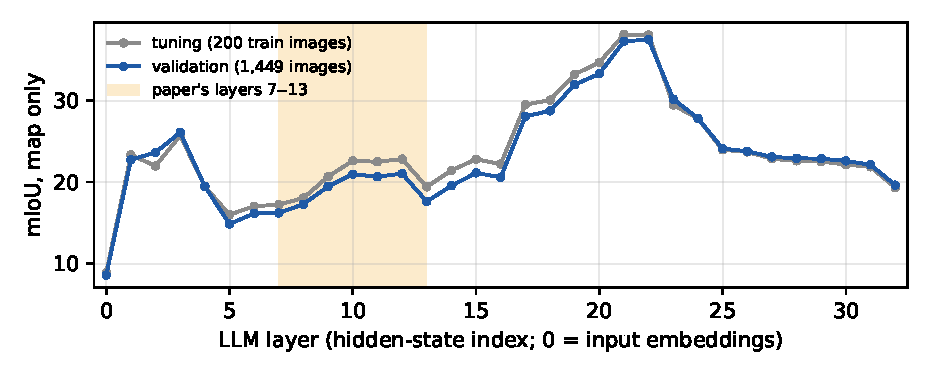
\includegraphics[width=0.85\linewidth]{layers.pdf}}{\textit{(pending)}}
\caption{VOC21 mIoU of the LLaVA map from a single layer, without SAM. Best single layer: \protectlayer 22 (37.5 mIoU).}
\label{fig:layers}
\end{figure}

\begin{table}[h]
\centering\small
\caption{Layer range of the similarity map: VOC21 mIoU of the map alone and of the full pipeline with SAM, against the
paper's Table 3 (full pipeline, validation).}
\label{tab:layers}
\begin{tabular}{lccccc}
\toprule
 & \multicolumn{2}{c}{Tuning (200)} & \multicolumn{2}{c}{Validation (1{,}449)} & Paper \\
Layers & map only & with SAM & map only & with SAM & with SAM \\
\midrule
\tabinput{tables/layer_ranges.tex}
\bottomrule
\end{tabular}
\end{table}

\begin{table}[h]
\centering\small
\caption{Foreground pixels labelled with the correct class: precision, recall, and the share of all pixels predicted as
foreground (ground truth: 27\%), \protectvalidation set.}
\label{tab:layerpr}
\begin{tabular}{llccc}
\toprule
Layers & Output & Precision & Recall & Predicted foreground \\
\midrule
\tabinput{tables/layer_precision.tex}
\bottomrule
\end{tabular}
\end{table}

\noindent With SAM, the layer ranges reproduce the paper's Table 3 closely (Table~\ref{tab:layers}): early ranges are
slightly worse, ranges around 7--13 are best, 15--22 loses about 20 points and 22--30 collapses. Ranges inside 7--17
are within about one point of each other, so the paper's 7--13 is a good but not uniquely best choice.

The map-only scores tell a different story (Figure~\ref{fig:layers}): a single layer's map is best in layers 17--22,
not in 7--13. Table~\ref{tab:layerpr} explains the difference. Middle-layer maps are small and precise: they mark only
about 5\% of the image, but 79\% of those pixels carry the right class. They miss most of each object, but they are
reliable \emph{seeds}, and SAM grows them into whole objects (precision 0.83, recall 0.67). Deeper maps cover more of the
object but also fire on wrong regions; the prompts derived from them produce oversized boxes, and SAM then marks 43\%
of the image as foreground (truth 27\%) at a precision of 0.50. The last layers respond almost everywhere. The paper's
observation that middle layers localize best therefore holds in a specific sense: they give the most \emph{precise}
class evidence, which is what a prompt-based segmenter needs, while coverage-oriented map quality peaks deeper.

\subsection{Attempts to improve the method}
Every attempt was evaluated on the 200-image tuning subset (Table~\ref{tab:tuning}); the reproduction scores 68.49
there. Each targeted a measured error source:
\begin{itemize}
\item \emph{False ``yes'' answers}: thresholds on LLaVA's probability of ``yes'' and an evidence filter. The filter drops
an unsure class whose map wins almost no area, and removes about half of the false positives at a small cost in true
classes.
\item \emph{Weak person maps}: a per-class or relative background threshold, and querying ``person, people''.
\item \emph{Several instances per class}: one SAM prompt per connected region.
\end{itemize}
None beat the reproduction clearly. Relative thresholds raised person IoU on the tuning set (24.4 to 45.0) but cost
more on other classes. Per-instance prompts let SAM answer small boxes with small masks and lost up to 41 points. The
only gain was a combination of three individually neutral changes (69.72, +1.23; bootstrap 95\% CI $-0.5$ to $+3.5$).
We fixed it before validation and ran it once, where it scored \textbf{65.69, i.e.\ $-0.15$ (95\% CI $-0.83$ to
$+0.55$)}. The tuning gain was sampling noise, so the final result is the plain reproduction. The paper's
$\alpha=0.75$, $\beta=0.19$ are also the best values in our grid.

\begin{table}[h]
\centering\small
\caption{Improvement attempts and hyperparameters on the 200-image tuning subset (reproduction: 68.49).}
\label{tab:tuning}
\begin{tabular}{lc}
\toprule
Change & mIoU \\
\midrule
\tabinput{tables/tuning.tex}
\bottomrule
\end{tabular}
\end{table}

\section{Qualitative results}
Figure~\ref{fig:success} shows typical successes: single objects and multi-class scenes are segmented with sharp
boundaries once SAM is prompted from LLaVA's partial maps. It also shows the off-by-one failure: the shifted state finds
the right region on easy images but misses or merges objects in crowded ones. Figure~\ref{fig:failures} shows the main
failure modes: close-up people reduced to faces, a person left out entirely in favour of an object LLaVA wrongly claims
(a boat on water), and a partially recovered table.

\begin{figure}[h]
\centering
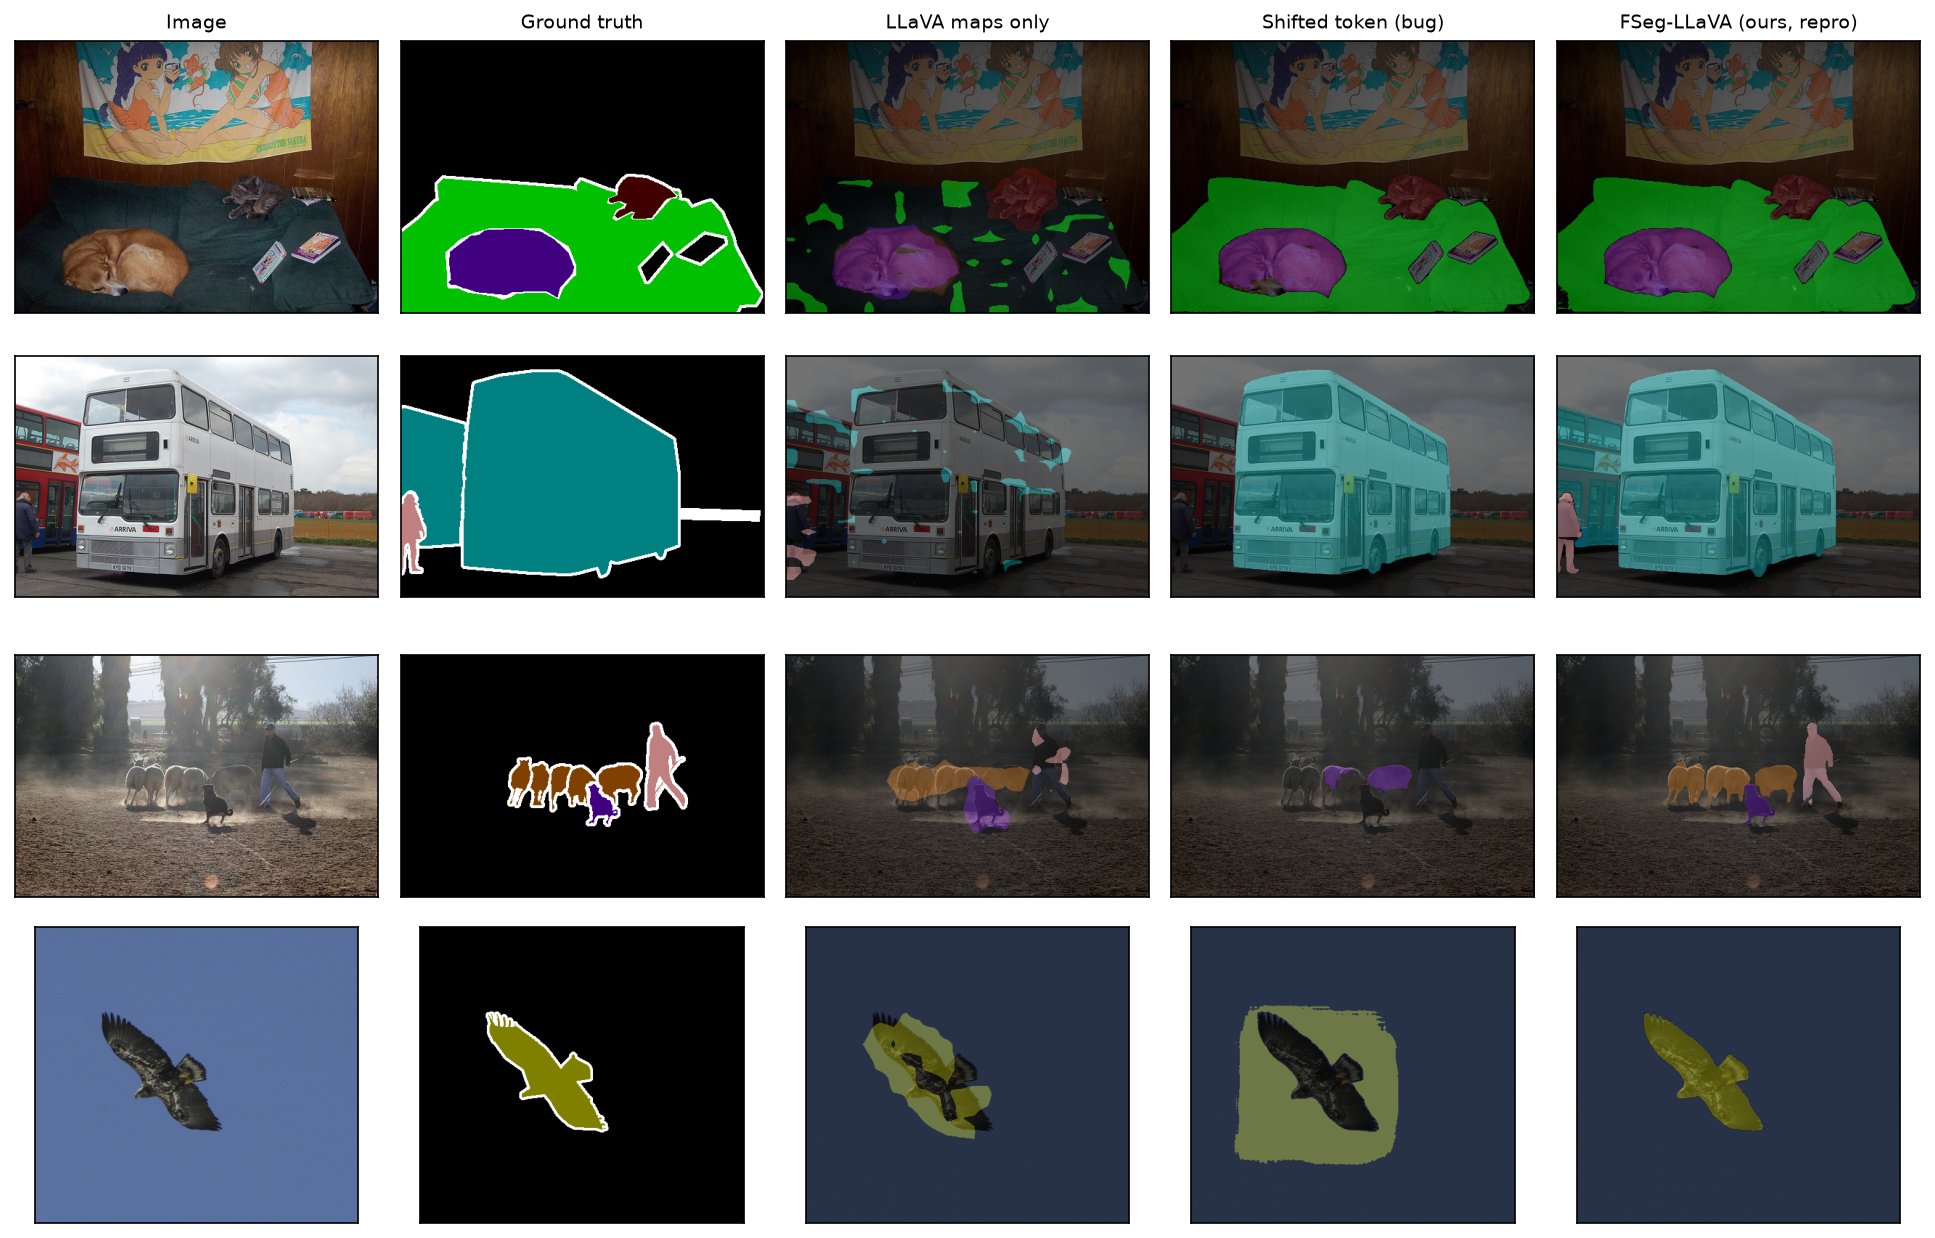
\includegraphics[width=\linewidth]{qualitative_success.png}
\caption{Validation examples. Columns: image, ground truth, LLaVA map only (no SAM), the off-by-one class-token
variant, and the reproduction.}
\label{fig:success}
\end{figure}

\begin{figure}[h]
\centering
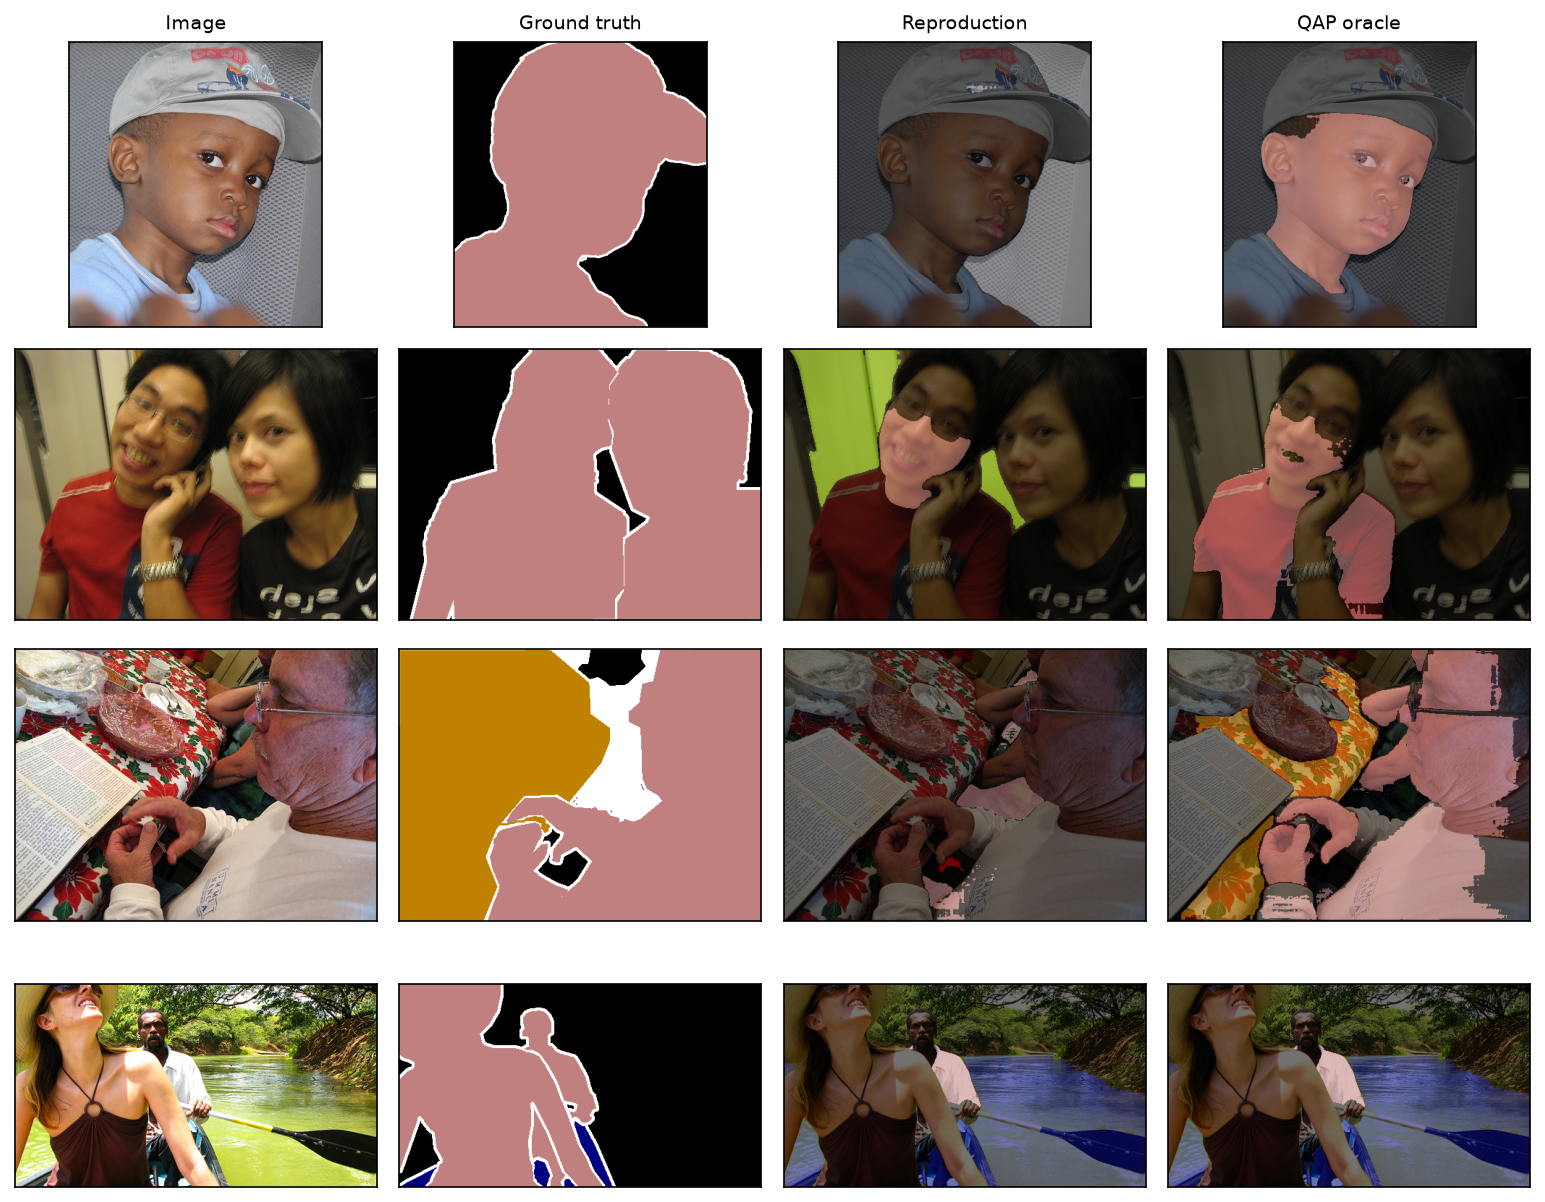
\includegraphics[width=0.85\linewidth]{qualitative_failures.png}
\caption{Validation failures involving people. Columns: image, ground truth, reproduction, oracle class list.}
\label{fig:failures}
\end{figure}

\section{Limitations}
\begin{itemize}
\item Only VOC 2012 was evaluated (the paper also reports COCO-Object, Context, COCO-Stuff and ADE20K), with one model
(LLaVA-1.5-7B). The LLaVA-1.6 13B variant needs about 48\,GB of GPU memory and does not fit our 24\,GB GPU.
\item Our port is not the authors' code; the 2.2-point gap to the paper is unexplained.
\item The tuning subset (200 images) is small; its bootstrap intervals span several points, which is why the one
apparent improvement did not transfer.
\item Runtime is dominated by one LLaVA generation per class: 20 queries per image (7\,s on an A30), so the method
scales poorly to large vocabularies, as the paper also notes.
\end{itemize}

\section{Conclusion}
The training-free method reproduces to within 2.2 mIoU of the paper on VOC 2012 using only frozen LLaVA and SAM. The
spatial signal inside LLaVA is real but coarse and narrowly located: it lives in the hidden state at the class token in
middle layers, alone gives under 20 mIoU, and becomes a competitive segmenter only as a prompt generator for SAM. The
remaining errors are mostly recognition errors in cluttered indoor scenes and weak localization of the generic word
``person''. Simple fixes for both did not hold up under a held-out evaluation.

\end{document}
